
	\section{Пространственная когерентность. Радиус пространственной когерентности,
		зависимость радиуса пространственной когерентности от угловых размеров
		источника света.}
	Будем рассматривать пространственную когерентность на примере опыта Юнга. \\
	 \begin{figure}[H]
	 	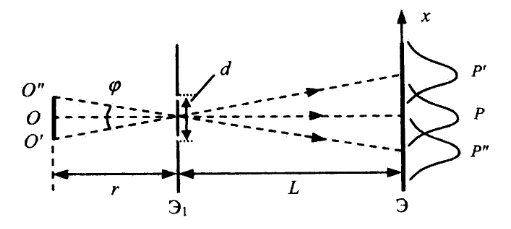
\includegraphics[scale = 0.6]{22_1}
	 \end{figure}
	 Пусть источник света имеет какие-то линейные размеры. Тогда каждая точка источника создает свою интерференционную картину, которые наслаиваются друг на друга. Как известно период полос $\dfrac{\lambda L}{d}$ а сдвиг за счет неточечности будет $\phi L$ итого получаем условие $b < \dfrac{\lambda}{\phi}$ это и называют радиусом когерентности. $ \rho = \dfrac{\lambda}{\phi}$
